\chapter{関連研究} \label{related}

この章では、既存のシミュレータを用いた教育の実例について紹介する。

\section{PhETの教育効果}


\subsection*{Ajrediniの 実験} \label{ajredini}

Ajredini~\cite{ajredini_real_2014} は、マケドニアの高校生に PhET を用いて電荷について教える実験を行った。実際の実験を行うグループ、PhET のシミュレーションを利用するグループ、実験を行わないグループの3つに分け、電荷に関する授業を行った。その後、いくつかのシチュエーションを指定し、スケッチを描かせた。各シチュエーションと正答率は表~\ref{ajredini_result}の通りであり、実際の実験と PhET との間の有意差は見られなかった。

\begin{table}[htb]
\noindent\rule{\linewidth}{0.4pt}
\begin{quote}
2つの軽い中性の金属球を糸でぶら下げる。次のような場合についてスケッチを描け。
\end{quote}
\begin{enumerate}
\renewcommand{\labelenumi}{\alph{enumi}).}
\item 両方の球体に毛布で擦ったプラスチック棒を接触させ、帯電させる
\item (a) の状態で、球体をより遠くに置く
\item 球体 A は毛布で擦ったプラスチック棒で帯電させ、球体 B は皮で擦ったガラス棒で帯電させる。
\item 両方の球体をプラスチック棒で帯電させるが、球体 A は球体 B より多く帯電させる。
\item 球体 A はプラスチック棒で帯電させ、球体 B は中性のままにする
\item 球体 A はガラス棒で帯電させ、球体 B は中性のままにする
\end{enumerate}
\centering
\begin{tabular}{rrrr}
  \toprule
  グループ & 実験 & PhET & 座学 \\
  \midrule
  a) & 75 & 66 & 43 \\
  b) & 35 & 34 & 14 \\
  c) & 67 & 70 & 31 \\
  d) & 23 & 26 & 12 \\
  e) and f) & 11 & 7 & 3 \\
  \bottomrule
\end{tabular}
\caption{Ajredini による実験の結果} \label{ajredini_result}
\end{table}

\subsection*{Prima の実験}

Prima~\cite{prima_learning_2018} は、インドネシアの中学生に PhET を用いて太陽系について教える実験を行った。PhET を用いるグループと用いないグループに分け授業を行い、その結果を Normalized Gain を用いて評価している。満点を $100$ とする pre-test と post-test の平均点をそれぞれ $\langle \textrm{pre\\-test} \rangle$, $\langle \textrm{post\\-test} \rangle$ とすると、 Normalized Gain $\langle g \rangle$ は以下のように求められる:
$$ \langle g \rangle = \dfrac{\langle \textrm{post\\-test} \rangle - \langle \textrm{pre\\-test} \rangle}{100 - \langle \textrm{pre\\-test} \rangle} $$
また、テストは Bloom's Taxonomy に基づき Remembering, Understanding, Applying, Analyzing の4領域で行われた。結果は表\ref{prima_table}の通りであり、全ての分野において PhET を用いた方が Normalized Gain が大きい。

\begin{table}[htb]
\centering
\begin{tabular}{lcccccc}
  \toprule
  \multirow{2}{*}{Cognitive level} & \multicolumn{3}{c}{Control Group} & \multicolumn{3}{c}{Experiment Group}\\
  \cmidrule(lr){2-4} \cmidrule(lr){5-7}
  & pretest & posttest & N-Gain & pretest & posttest & N-Gain\\
  \midrule
  Remembering (C1) & 33.33 & 76.19 & 0.64 & 44.44 & 84.12 & 0.71\\
  Understanding (C2) & 38.62 & 57.67 & 0.31 & 51.85 & 75.66 & 0.49\\
  Applying (C3) & 54.76 & 80.95 & 0.57 & 69.04 & 92.85 & 0.76\\
  Analyzing (C4) & 56.34 & 75.39 & 0.43 & 57.14 & 80.15 & 0.53\\
  \bottomrule
\end{tabular}

\caption{Primaによる実験の結果}
\label{prima_table}
\end{table}

\subsection*{Rehman の実験}
Rehman~\cite{rehman_teaching_2021} は、パキスタンの高校生に PhET を用いて重さと質量の概念について教える実験を行った。また、この授業は週5回・1ヶ月間行われた。結果は表~\ref{rehman_result}の通りであり、有意差が認められる。

\begin{table}[htb]
\centering
\begin{tabular}{lcccccc}
\toprule
& Control Group & Experiment Group \\
\midrule
pretest & 11.82 & 12.68 \\
posttest & 16.84 & 29.46 \\
\bottomrule
\end{tabular}
\caption{Rehman による実験の結果} \label{rehman_result}
\end{table}

% \section{Modellus Software}
% Modellus~\cite{modellus} は、数学と物理学のためのモデリングツールである。Modellus を用いる事で、学習者や教育者はインタラクティブにモデルを作成できる。また、モデルの設定はプログラミング言語や特別なコマンドを必要とせず、従来の数式で可能であるという点で \simname とよく似ている。しかし、

\section{Excel を用いる例}

Uddin ら~\cite{uddin_teaching_2017}は、Microsoft Excel を用いて物理系を定義・可視化する手法を提案した。この手法では、自由に方程式を定義することが可能であるが、単位の異なる足し算などの不正な計算をしてしまっても気づくことができない。また、Excel 上で表現された数式は実際の数式と視覚的に遠い。例えば、風速の分布を描画する例でワイブル分布 $f(t) = \dfrac{m}{\eta}\left(\dfrac{t}{\eta}\right)^{m-1}\exp{\left\{-\left(\dfrac{t}{\eta}\right)^m\right\}}$ を用いているが、Excel 上でのこの関数の表現は ((H\$1/H\$2) * ((C3/H\$2)\^{}(H\$1-1)) * EXP(-((C3/H\$2)\^{}H\$1))) となっている。そのため、これを見てもワイブル分布であるとはわかりにくい。

\section{Easy Java Simulations}
Easy Java Simulations~\cite{christian_modeling_2007} は、ユーザが入力した数式をもとにシミュレーションを生成してくれる Java のソフトウェアである。シミュレーションの科学的な側面にほとんどの時間を集中させ、その他の必要なタスクをコンピュータに自動的に行わせるように設計されている。
Easy Java Simulations は、ユーザ自身がシミュレーションを作成できるという点で \simname と類似している。 \simname には動作例が存在し、次元のチェックを行うため、学習者が物理系を作成した際により誤りに気づきやすいと考えられる。

\begin{figure}[htb]
  \centering
  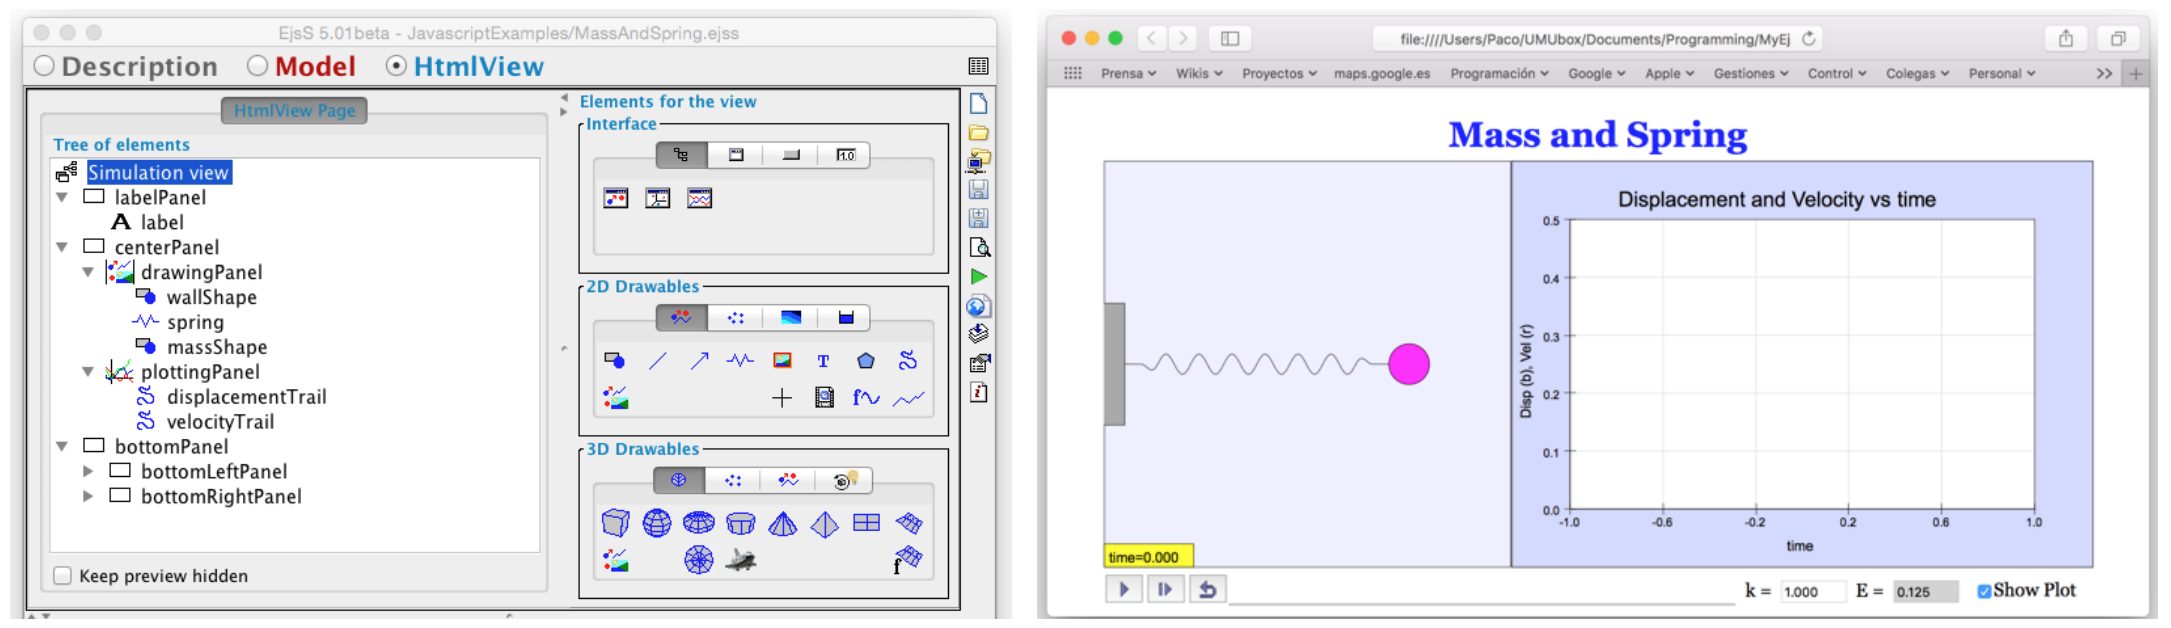
\includegraphics[width=0.9\linewidth]{work/ejs_example.png}
  \caption{Easy Java Simulations で作成したシミュレーションの例~\cite{esquembre_easy_2019}}
\end{figure}
